\section{Introduzione}\label{sec:Introduzione}
Questo elaborato rappresenta la relazione del progetto svolto per l'esame di Ingegneria del Software del corso di Laurea Triennale in Ingegneria Informatica dell'Università degli Studi di Firenze.
Il codice sorgente del progetto è disponibile su \textit{GitHub} al seguente indirizzo: \href{https://github.com/TommyAen/SWE-Project}{SWE-Project}.
\subsection{Statement}
Questo progetto si propone di sviluppare un'applicazione per la gestione e l'utilizzo di servizi di carsharing universitario: l'università mette a disposizione delle navette che possono essere usate dagli studenti per muoversi tra sedi universitarie in modo efficiente e sostenibile.
\newline
L'applicazione sarà usata dagli studenti per la prenotazione di viaggi in qualità di passeggeri o guidatori, e dagli amministratori per la gestione delle risorse.
Il sistema deve permettere la registrazione e autenticazione di studenti o admin all'applicativo, e la possibilità di prenotare e visualizzare i viaggi.
Il progetto trae ispirazione da TUSS (\href{https://www.tuss.unifi.it/}{The Ultimate Sharing Service}) dell'Università di Firenze, un servizio sviluppato per offrire una soluzione concreta alle difficoltà di spostamento tra le diverse sedi universitarie.
\subsection{Architettura e pratiche utilizzate}
Il software è stato sviluppato in Java, con il supporto di un database PostgreSQL per la memorizzazione e la gestione persistente dei dati. Per la connessione tra l’applicazione e il database è stata utilizzata la libreria JDBC (Java DataBase Connectivity).\\
\noindent
Per garantire una chiara separazione delle responsabilità l'architettura del progetto è stata suddivisa in tre macro-componenti principali: Domain Model, Business Logic e ORM. Ciascun package ha un ruolo ben definito:
\begin{itemize}
\item \textbf{Domain Model}: definisce le entità principali del dominio dell'applicazione
\item \textbf{ORM}: include le classi responsabili del mapping tra oggetti Java e tabelle del database, permettendo la lettura e scrittura dei dati in modo astratto
\item \textbf{Business Logic}: comprende le classi che gestiscono le regole di funzionamento dell'applicazione, coordinando le operazioni tra il dominio e la persistenza dei dati, come la prenotazione dei viaggi e la verifica dei permessi.
\end{itemize}
\begin{figure}
    \centering
    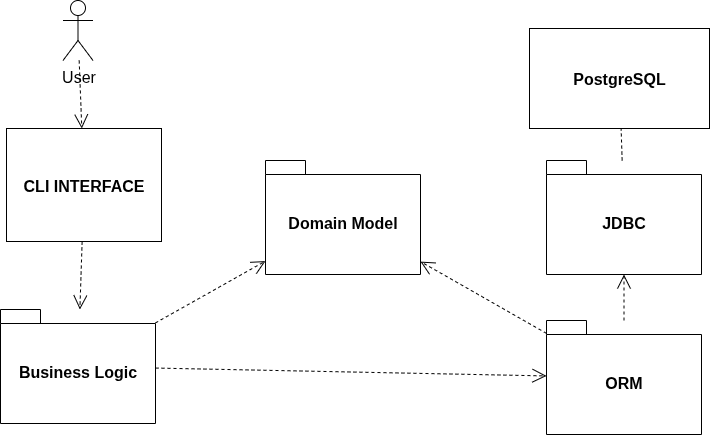
\includegraphics[width=1\linewidth]{Images/PkgDeps.png}
    \caption{Package Dependency Diagram}
    \label{fig:pkdep}
\end{figure}
I diagrammi UML, inclusi gli Use Case Diagram e i Class Diagram, sono stati realizzati seguendo lo standard UML (Unified Modeling Language).\\
\noindent Di seguito l’elenco degli strumenti e delle piattaforme utilizzati durante lo sviluppo:
\begin{itemize}
\item \textbf{IntelliJ IDEA}: IDE utilizzato per lo sviluppo in Java
\item \textbf{PgAdmin}: interfaccia grafica per la gestione di database PostgreSQL
\item \textbf{GitHub}: piattaforma per il versionamento e la condivisione del codice sorgente
\item \textbf{draw.io}: utilizzato per la realizzazione del navigation diagram e dei diagrammi UML
\item \textbf{Figma}: software per la creazione di mock-up
\item \textbf{Overleaf.com}: piattaforma per la stesura collaborativa del report in \LaTeX
\end{itemize}
\newpage